\chapter{Thử nghiệm hệ thống}

Để chứng minh tính đúng đắn của hệ thống, tôi thực hiện thử nghiệm hệ thống với một câu truy vấn: Liệt kê các thiết bị trong trung tâm HPCC. \\

Câu truy vấn tương ứng trong hệ thống của tôi là:
\begin{figure}
	\center
	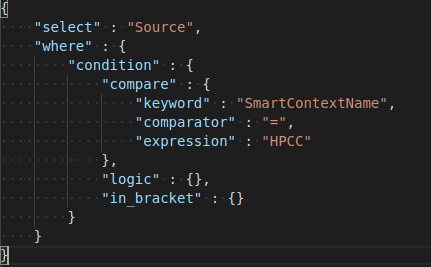
\includegraphics[scale=0.5]{image/demo_query}
	\caption{Câu truy vấn thực nghiệm}
\end{figure}

Kết quả thu được là :\\


TODO\\
TODO \\
TODO\\
TODO\\
TODO\\
TODO\\
TODO\\
TODO\\



Để chứng minh hệ thống có tính khả mở, tôi thêm một nền tảng IoT là ThingsBoard vào hệ thống bằng việc viết thêm một driver để ánh xạ dữ liệu từ định dạng của ThingsBoard về định dạng của ontology. Tôi sẽ thực hiện câu truy vấn: Lấy tất cả các platform có trong trung tâm HPCC để chứng minh đã thêm được ThingsBoard vào hệ thống. \\

Câu truy vấn tương ứng trong hệ thống là:
\begin{figure}
	\center
	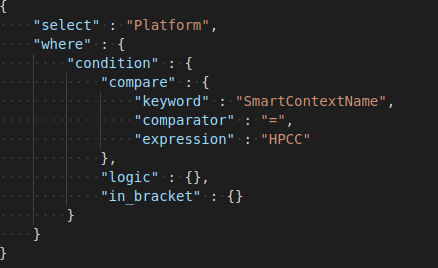
\includegraphics[scale=0.5]{image/add_thingsboard}
	\caption{Thêm ThingsBoard vào hệ thống}
\end{figure}

Kết quả thu được trước khi thêm Thingsboard: \\


TODO\\
TODO \\
TODO\\
TODO\\
TODO\\
TODO\\
TODO\\
TODO\\



Kết quả thu được sau khi thêm Thingsboard:\\


TODO\\
TODO \\
TODO\\
TODO\\
TODO\\
TODO\\
TODO\\
TODO\\

